%% ========================================================================
%% Biodata Penulis
%% ========================================================================

\chapter*{Biodata Penulis}
\addcontentsline{toc}{chapter}{Biodata Penulis}

%% ---- Sofyan Noor Arief ------------------------------------------------
\begin{wrapfigure}{l}{2.6cm}
    \vspace{-\baselineskip}
    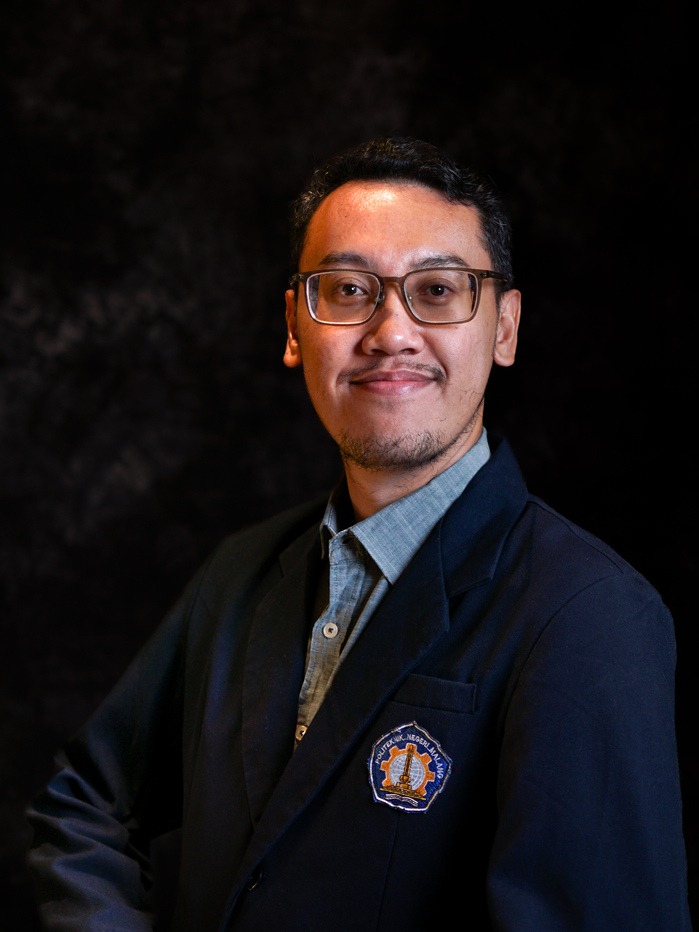
\includegraphics[width=2.4cm]{docs/sofyan.jpg}
    \vspace{-\baselineskip}
\end{wrapfigure}
\small\noindent\textbf{Sofyan Noor Arief} adalah dosen junior di Jurusan Teknologi
Informasi Politeknik Negeri Malang, dengan fokus keilmuan pada bidang jaringan
komputer. Di luar kegiatan mengajar, ia aktif sebagai konsultan dan teknisi
pemasangan jaringan secara lepas. Menyelesaikan studi D3 Manajemen Informatika di
POLINEMA, dilanjutkan D4 Lintas Jalur Teknik Informatika di PENS, kemudian meraih
gelar magister dari Program Studi Teknik Informatika Institut Teknologi Sepuluh
Nopember (ITS) Surabaya. Minat risetnya berpusat pada \textit{distributed computing}
yang diimplementasikan pada perangkat \textit{low-power computing}. Penulis dapat
dihubungi melalui \texttt{sofyan@polinema.ac.id}.
\par\medskip
\noindent\rule{\linewidth}{0.4pt}
\par\medskip

%% ---- Dian Hanifudin Subhi --------------------------------------------
\begin{wrapfigure}{l}{2.6cm}
    \vspace{-\baselineskip}
    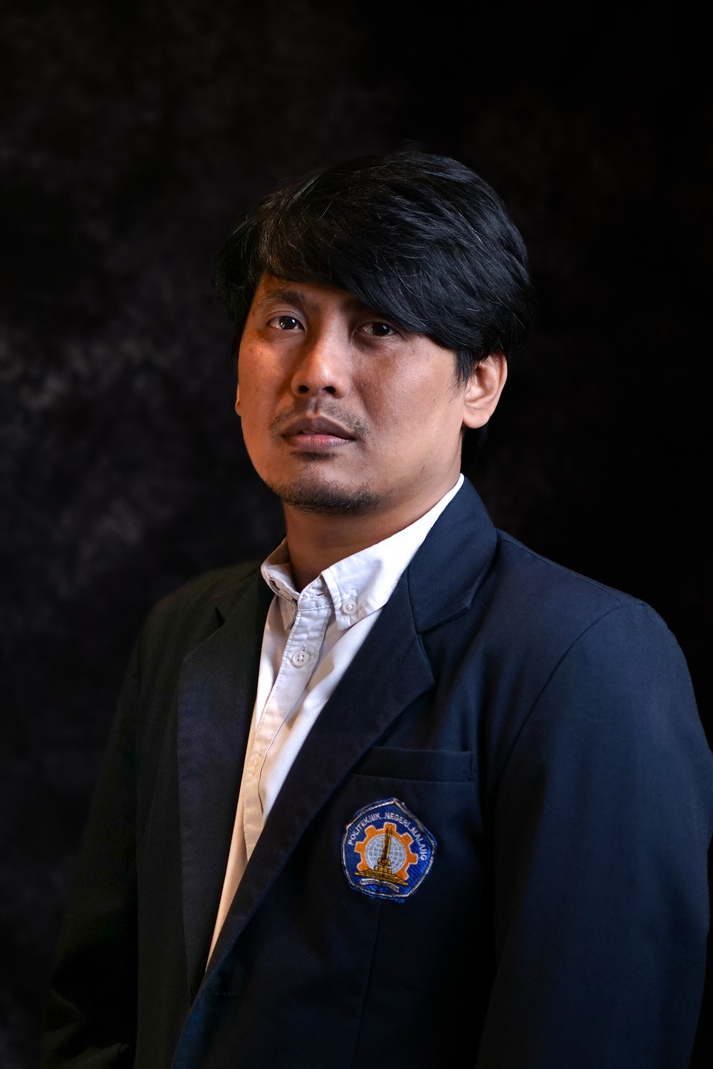
\includegraphics[width=2.4cm]{docs/subhi.jpg}
    \vspace{-\baselineskip}
\end{wrapfigure}
\small\noindent\textbf{Dian Hanifudin Subhi} adalah dosen Teknologi Informasi di
Politeknik Negeri Malang yang menjalani dua peran sekaligus: pengajar di ruang
kuliah dan praktisi yang terlibat langsung dalam pengembangan produk serta layanan
digital. Menyelesaikan pendidikan S1 dan S2 di Institut Teknologi Sepuluh Nopember
(ITS) Surabaya, ia membawa bekal akademik yang kuat ke dalam praktik industri nyata.
Keahliannya berpusat pada pemrograman, \textit{Quality Assurance} (QA), dan
\textit{cloud computing}: mulai dari pengembangan aplikasi, penerapan strategi
pengujian yang terukur, hingga pembangunan layanan yang siap beroperasi di lingkungan
\textit{cloud} skala produksi. Pembaca yang ingin mengikuti perkembangan karyanya
atau berdiskusi tentang teknologi dapat mengunjungi \texttt{dhanifudin.com}.
\par\medskip
\noindent\rule{\linewidth}{0.4pt}
\par\medskip

%% ---- Muhammad Afif Hendrawan ----------------------------------------
\begin{wrapfigure}{l}{2.6cm}
    \vspace{-\baselineskip}
    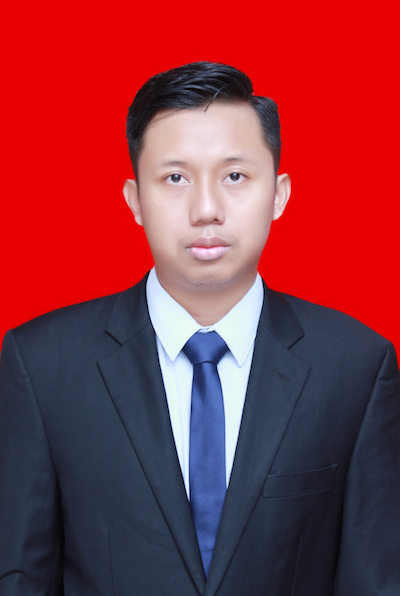
\includegraphics[width=2.4cm]{docs/afif.jpg}
    \vspace{-\baselineskip}
\end{wrapfigure}
\small\noindent\textbf{Muhammad Afif Hendrawan} adalah pengajar di bidang teknologi
informasi dengan latar belakang keilmuan kecerdasan buatan. Menyelesaikan pendidikan
sarjana di Departemen Sistem Informasi Institut Teknologi Sepuluh Nopember, kemudian
melanjutkan studi magister di Departemen Teknik Elektro institusi yang sama. Dalam
kegiatan akademik, ia aktif menyusun materi pembelajaran dan mengembangkan pendekatan
praktis agar konsep-konsep komputasi, pengolahan data, dan kecerdasan buatan dapat
dipahami serta diterapkan secara efektif oleh pembaca.
\par\medskip
\noindent\rule{\linewidth}{0.4pt}
\par\medskip

%% ---- Irsyad Arif Mashudi --------------------------------------------
\begin{wrapfigure}{l}{2.6cm}
    \vspace{-\baselineskip}
    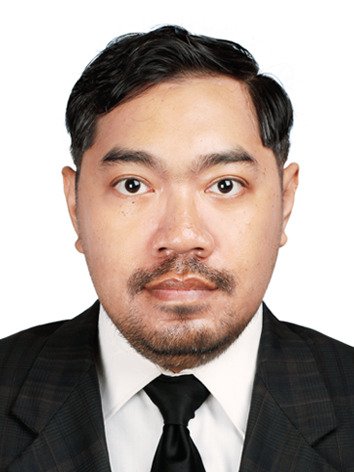
\includegraphics[width=2.4cm]{docs/irsyad.jpg}
    \vspace{-\baselineskip}
\end{wrapfigure}
\small\noindent\textbf{Irsyad Arif Mashudi} adalah pengajar di Politeknik Negeri
Malang yang menaruh minat pada perkembangan teknologi informasi. Menyelesaikan
studi sarjana dan magister di Institut Teknologi Sepuluh Nopember (ITS), ia kini
aktif mendampingi pembaca dalam mempelajari rekayasa perangkat lunak serta sistem
jaringan komputer. Di sela aktivitas akademik, Irsyad menekuni riset di bidang
sistem cerdas sekaligus meluangkan waktu untuk membantu proses digitalisasi di
berbagai sekolah dan lembaga sosial di sekitarnya.
\par\medskip
\noindent\rule{\linewidth}{0.4pt}
\par\medskip

%% ---- Luqman Affandi -------------------------------------------------
\begin{wrapfigure}{l}{2.6cm}
    \vspace{-\baselineskip}
    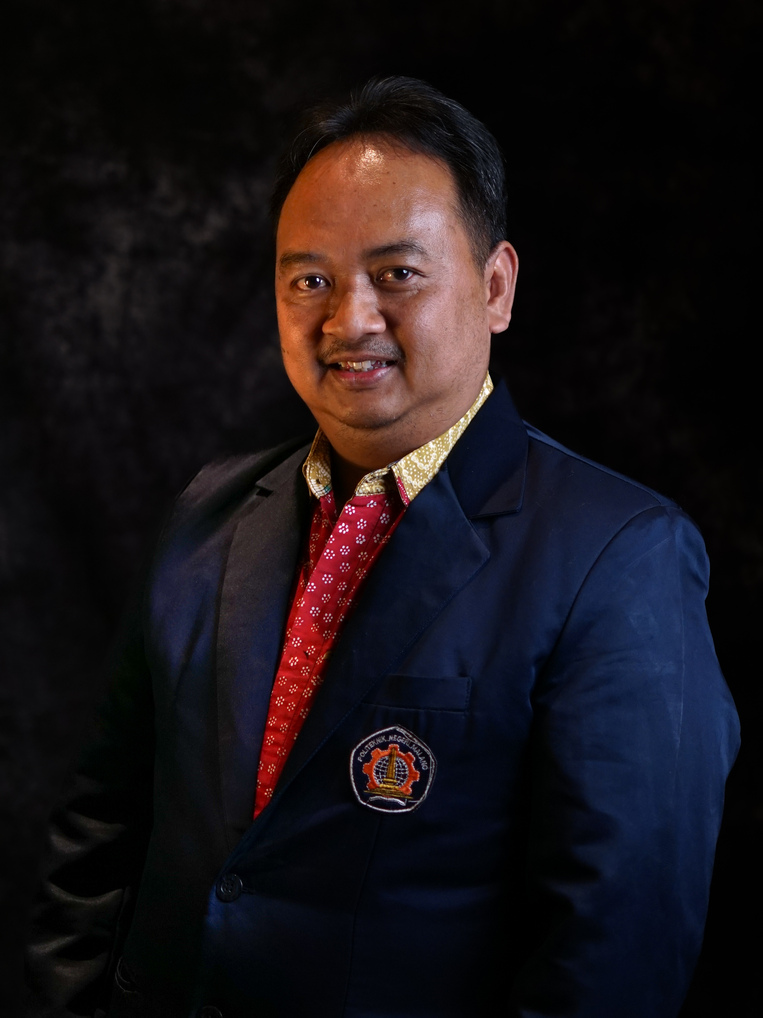
\includegraphics[width=2.4cm]{docs/luqman.jpg}
    \vspace{-\baselineskip}
\end{wrapfigure}
\small\noindent\textbf{Luqman Affandi} adalah dosen tetap berstatus PNS di Jurusan
Teknologi Informasi Politeknik Negeri Malang, saat ini menjabat sebagai Sekretaris
Jurusan. Menyelesaikan S1 Teknik Informatika di STMIK PPKIA Pradnya Paramita Malang,
S2 Magister Sistem Informasi di Universitas Gunadarma Jakarta, dan kini sedang
menempuh program doktoral di bidang Teknik Elektro dan Informatika di Universitas
Negeri Malang. Perjalanan kepemimpinannya mencakup jabatan Ketua STMIK PPKIA Pradnya
Paramita Malang serta Ketua Program Studi D3 Manajemen Informatika PSDKU Polinema
Pamekasan. Selain mengampu mata kuliah sistem operasi, jaringan komputer, dan
keamanan jaringan, ia memegang sejumlah sertifikasi internasional di bidang basis
data, keamanan sistem informasi, dan pemrograman. Fokus riset saat ini adalah
kompresi data dan teknologi data.

\cleardoublepage
